\PassOptionsToPackage{unicode=true}{hyperref} % options for packages loaded elsewhere
\PassOptionsToPackage{hyphens}{url}
%
\documentclass[russian,ignorenonframetext,]{beamer}
\usepackage{pgfpages}
\setbeamertemplate{caption}[numbered]
\setbeamertemplate{caption label separator}{: }
\setbeamercolor{caption name}{fg=normal text.fg}
\beamertemplatenavigationsymbolsempty
\usepackage{lmodern}
\usepackage{amssymb,amsmath}
\usepackage{ifxetex,ifluatex}
\usepackage{fixltx2e} % provides \textsubscript
\ifnum 0\ifxetex 1\fi\ifluatex 1\fi=0 % if pdftex
  \usepackage[T1]{fontenc}
  \usepackage[utf8]{inputenc}
  \usepackage{textcomp} % provides euro and other symbols
\else % if luatex or xelatex
  \usepackage{unicode-math}
  \defaultfontfeatures{Ligatures=TeX,Scale=MatchLowercase}
\fi
\usetheme[]{metropolis}
% use upquote if available, for straight quotes in verbatim environments
\IfFileExists{upquote.sty}{\usepackage{upquote}}{}
% use microtype if available
\IfFileExists{microtype.sty}{%
\usepackage[]{microtype}
\UseMicrotypeSet[protrusion]{basicmath} % disable protrusion for tt fonts
}{}
\IfFileExists{parskip.sty}{%
\usepackage{parskip}
}{% else
\setlength{\parindent}{0pt}
\setlength{\parskip}{6pt plus 2pt minus 1pt}
}
\usepackage{hyperref}
\hypersetup{
            pdftitle={Применение искусственных нейронных сетей для поиска клонов в исходном коде программ},
            pdfauthor={Арсений Зорин; 23541/3},
            pdfborder={0 0 0},
            breaklinks=true}
\urlstyle{same}  % don't use monospace font for urls
\newif\ifbibliography
\usepackage{longtable,booktabs}
\usepackage{caption}
% These lines are needed to make table captions work with longtable:
\makeatletter
\def\fnum@table{\tablename~\thetable}
\makeatother
\usepackage{graphicx,grffile}
\makeatletter
\def\maxwidth{\ifdim\Gin@nat@width>\linewidth\linewidth\else\Gin@nat@width\fi}
\def\maxheight{\ifdim\Gin@nat@height>\textheight\textheight\else\Gin@nat@height\fi}
\makeatother
% Scale images if necessary, so that they will not overflow the page
% margins by default, and it is still possible to overwrite the defaults
% using explicit options in \includegraphics[width, height, ...]{}
\setkeys{Gin}{width=\maxwidth,height=\maxheight,keepaspectratio}
% Prevent slide breaks in the middle of a paragraph:
\widowpenalties 1 10000
\raggedbottom
\setbeamertemplate{part page}{
\centering
\begin{beamercolorbox}[sep=16pt,center]{part title}
  \usebeamerfont{part title}\insertpart\par
\end{beamercolorbox}
}
\setbeamertemplate{section page}{
\centering
\begin{beamercolorbox}[sep=12pt,center]{part title}
  \usebeamerfont{section title}\insertsection\par
\end{beamercolorbox}
}
\setbeamertemplate{subsection page}{
\centering
\begin{beamercolorbox}[sep=8pt,center]{part title}
  \usebeamerfont{subsection title}\insertsubsection\par
\end{beamercolorbox}
}
\AtBeginPart{
  \frame{\partpage}
}
\AtBeginSection{
  \ifbibliography
  \else
    \frame{\sectionpage}
  \fi
}
\AtBeginSubsection{
  \frame{\subsectionpage}
}
\setlength{\emergencystretch}{3em}  % prevent overfull lines
\providecommand{\tightlist}{%
  \setlength{\itemsep}{0pt}\setlength{\parskip}{0pt}}
\setcounter{secnumdepth}{0}

% set default figure placement to htbp
\makeatletter
\def\fps@figure{htbp}
\makeatother

\renewcommand{\caption}[1]{}
\setsansfont[Scale=1.10]{SF Pro Text}
\setmonofont[Scale=0.95]{Liberation Mono}
\metroset{outer/numbering=fraction}
\metroset{titleformat=regular}
\graphicspath{{pics/}}
\ifnum 0\ifxetex 1\fi\ifluatex 1\fi=0 % if pdftex
  \usepackage[shorthands=off,main=russian]{babel}
\else
  % load polyglossia as late as possible as it *could* call bidi if RTL lang (e.g. Hebrew or Arabic)
  \usepackage{polyglossia}
  \setmainlanguage[]{russian}
\fi

\title{Применение искусственных нейронных сетей для поиска клонов в исходном
коде программ}
\author{Студент гр. 23541/3 : Зорин А.Г.\\Научный руководитель: Ицыксон В.М}
\institute{\center{09.04.01.15: Технологии проектирования системного и прикладного программного обеспечения\\Санкт-Петербургский политехнический университет Петра Великого\\Институт компьютерных наук и технологий\\Кафедра <<Компьютерные системы и программные технологии>>}}
\date{\today}

\begin{document}
\frame{\titlepage}

\begin{frame}{Что такое клон?}
\protect\hypertarget{ux447ux442ux43e-ux442ux430ux43aux43eux435-ux43aux43bux43eux43d}{}

\textbf{Программные клоны} --- повторяющиеся или похожие фрагменты
исходного кода программы

\end{frame}

\begin{frame}{Причины возникновения}
\protect\hypertarget{ux43fux440ux438ux447ux438ux43dux44b-ux432ux43eux437ux43dux438ux43aux43dux43eux432ux435ux43dux438ux44f}{}

\begin{itemize}
\tightlist
\item
  Копирование кода
\item
  Генерация кода
\item
  Преодоление различных ограничений
\item
  Использование шаблонов
\end{itemize}

\end{frame}

\begin{frame}{Недостатки клонов}
\protect\hypertarget{ux43dux435ux434ux43eux441ux442ux430ux442ux43aux438-ux43aux43bux43eux43dux43eux432}{}

\begin{itemize}
\tightlist
\item
  Увеличение сложности поддержки и развития проекта
\item
  Увеличение размера проекта
\item
  Распространение ошибок
\end{itemize}

\end{frame}

\begin{frame}{Типы клонов}
\protect\hypertarget{ux442ux438ux43fux44b-ux43aux43bux43eux43dux43eux432}{}

\begin{figure}
\centering
\includegraphics{clones1}
\caption{clones}
\end{figure}

\end{frame}

\begin{frame}{Типы клонов}
\protect\hypertarget{ux442ux438ux43fux44b-ux43aux43bux43eux43dux43eux432-1}{}

\begin{figure}
\centering
\includegraphics{clones2}
\caption{clones}
\end{figure}

\end{frame}

\begin{frame}{Методы обнаружения клонов}
\protect\hypertarget{ux43cux435ux442ux43eux434ux44b-ux43eux431ux43dux430ux440ux443ux436ux435ux43dux438ux44f-ux43aux43bux43eux43dux43eux432}{}

\begin{itemize}
\tightlist
\item
  Анализ текста
\item
  Анализ токенов
\item
  Анализ синтаксических деревьев
\item
  Анализ графов
\item
  Анализ метрик
\item
  Гибридные методы
\end{itemize}

\end{frame}

\begin{frame}{Использование нейронных сетей}
\protect\hypertarget{ux438ux441ux43fux43eux43bux44cux437ux43eux432ux430ux43dux438ux435-ux43dux435ux439ux440ux43eux43dux43dux44bux445-ux441ux435ux442ux435ux439}{}

\begin{figure}
\centering
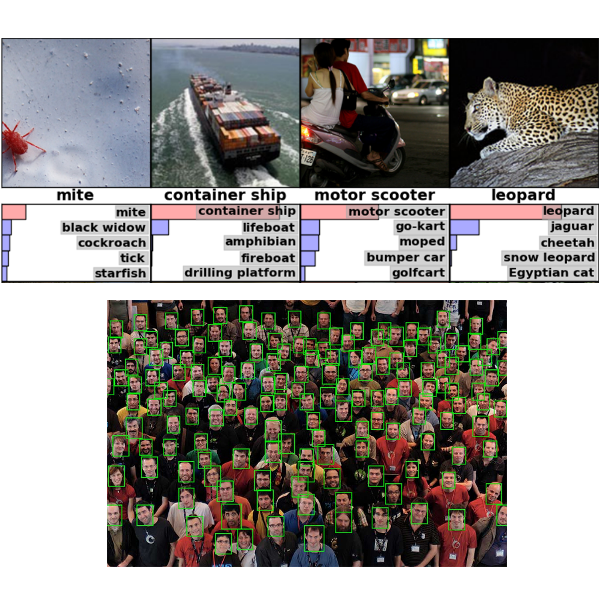
\includegraphics{merge}
\caption{Usage}
\end{figure}

\end{frame}

\begin{frame}{Что такое РНC?}
\protect\hypertarget{ux447ux442ux43e-ux442ux430ux43aux43eux435-ux440ux43dc}{}

\textbf{Рекуррентная нейронная сеть (РНС)} --- это сеть, в которой
нейроны получают информацию не только от предыдущего слоя, но и
информацию о предыдущем состоянии текущего слоя

\begin{figure}
\centering
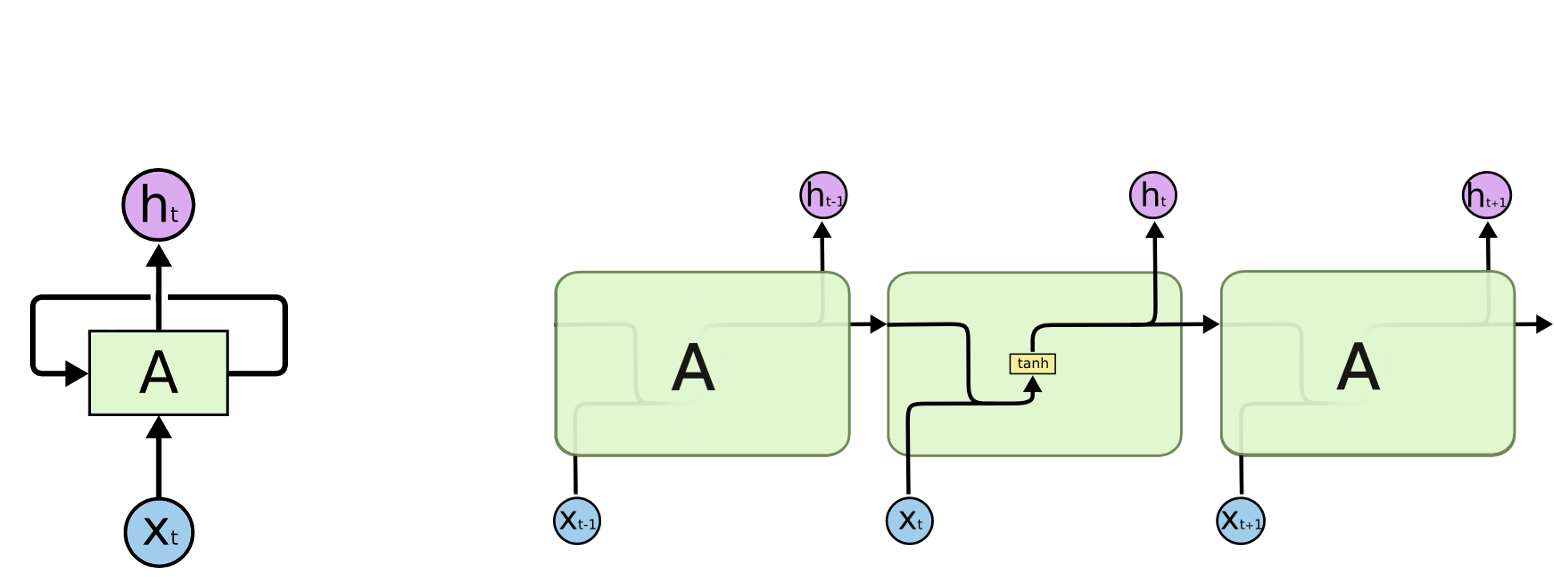
\includegraphics{rnn}
\caption{RNN}
\end{figure}

\end{frame}

\begin{frame}{Причины выбора РНС}
\protect\hypertarget{ux43fux440ux438ux447ux438ux43dux44b-ux432ux44bux431ux43eux440ux430-ux440ux43dux441}{}

\begin{itemize}
\tightlist
\item
  Анализ контекста
\item
  Распознавание образов
\item
  Определение сходства
\item
  И т.д.
\end{itemize}

\end{frame}

\begin{frame}{Выбранная архитектура}
\protect\hypertarget{ux432ux44bux431ux440ux430ux43dux43dux430ux44f-ux430ux440ux445ux438ux442ux435ux43aux442ux443ux440ux430}{}

\begin{figure}
\centering

\includegraphics{siam}
\caption{siam}
\end{figure}

\end{frame}

\begin{frame}{Этапы}
\protect\hypertarget{ux44dux442ux430ux43fux44b}{}

\begin{figure}
\centering
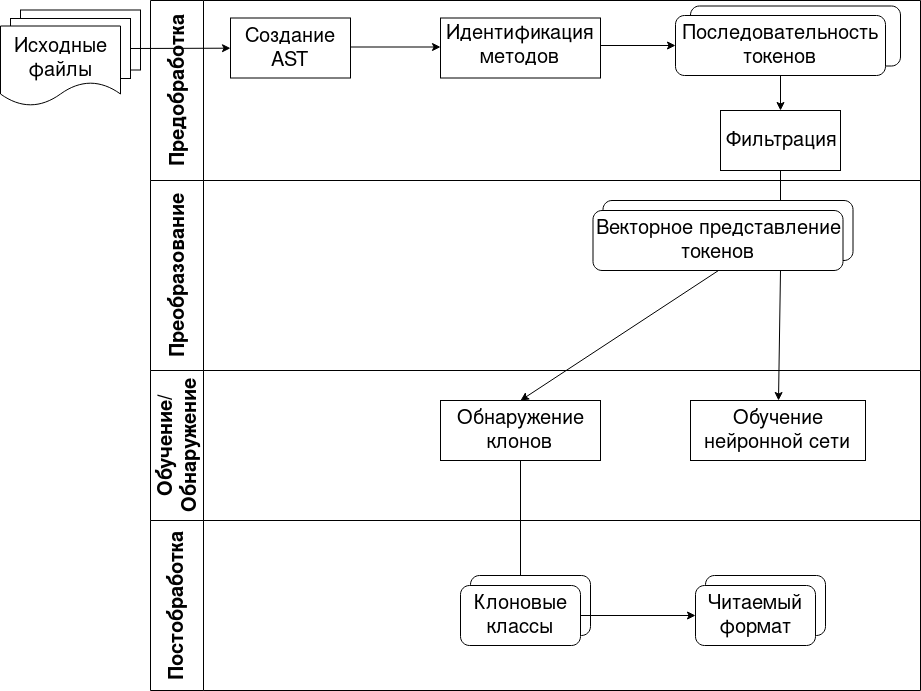
\includegraphics{struct}
\caption{stages}
\end{figure}

\end{frame}

\begin{frame}{Обучающая выборка данных}
\protect\hypertarget{ux43eux431ux443ux447ux430ux44eux449ux430ux44f-ux432ux44bux431ux43eux440ux43aux430-ux434ux430ux43dux43dux44bux445}{}

\begin{itemize}
\tightlist
\item
  Искусственные клоны
\item
  BigCloneBench
\end{itemize}

\end{frame}

\begin{frame}{Генерация данных}
\protect\hypertarget{ux433ux435ux43dux435ux440ux430ux446ux438ux44f-ux434ux430ux43dux43dux44bux445}{}

\begin{figure}
\centering
\includegraphics{mut_stages}
\caption{mutator}
\end{figure}

\end{frame}

\begin{frame}{BigCloneBench}
\protect\hypertarget{bigclonebench}{}

\begin{itemize}
\tightlist
\item
  25 тыс. проектов на Java
\item
  6.3 млн. клоновых пар
\item
  262.5 тыс. неклоновых пар
\end{itemize}

\end{frame}

\begin{frame}{Результаты: искусственные клоны}
\protect\hypertarget{ux440ux435ux437ux443ux43bux44cux442ux430ux442ux44b-ux438ux441ux43aux443ux441ux441ux442ux432ux435ux43dux43dux44bux435-ux43aux43bux43eux43dux44b}{}

\begin{longtable}[]{@{}ccccccc@{}}
\toprule
Methods & KLOC & Clones & R, \% & P, \% & F1, \% & Time,
min\tabularnewline
\midrule
\endhead
3951 & 195 & 1348 & 73 & 76 & 74 & 06:31\tabularnewline
7954 & 679 & 4731 & 77 & 73 & 75 & 09:28\tabularnewline
12573 & 2803 & 24385 & 75 & 73 & 74 & 14:44\tabularnewline
20842 & 2947 & 32679 & 74 & 75 & 75 & 17:37\tabularnewline
\bottomrule
\end{longtable}

\begin{itemize}
\tightlist
\item
  Средняя точность: 74.5\%
\item
  Средняя скорость анализа: 14.35 метод/сек
\end{itemize}

\end{frame}

\begin{frame}{Результаты: BigCloneBench}
\protect\hypertarget{ux440ux435ux437ux443ux43bux44cux442ux430ux442ux44b-bigclonebench}{}

\begin{longtable}[]{@{}ccccccc@{}}
\toprule
Methods & KLOC & Clones & R, \% & P, \% & F1, \% & Time,
min\tabularnewline
\midrule
\endhead
4092 & 228 & 1697 & 94 & 97 & 95 & 04:42\tabularnewline
8270 & 768 & 5453 & 88 & 94 & 91 & 06:55\tabularnewline
10892 & 3192 & 32041 & 88 & 93 & 90 & 09:44\tabularnewline
19711 & 2830 & 24797 & 90 & 76 & 82 & 14:43\tabularnewline
\bottomrule
\end{longtable}

\begin{itemize}
\tightlist
\item
  Средняя точность: 89.5\%
\item
  Средняя скорость анализа: 14.35 метод/сек
\end{itemize}

\end{frame}

\begin{frame}{Сравнение с имеющимися инструментами\footnote<.->{J.
  Svajlenko and C. K. Roy, ``Evaluating clone detection tools with
  BigCloneBench'', 2015 ICSME, Bremen}}
\protect\hypertarget{ux441ux440ux430ux432ux43dux435ux43dux438ux435-ux441-ux438ux43cux435ux44eux449ux438ux43cux438ux441ux44f-ux438ux43dux441ux442ux440ux443ux43cux435ux43dux442ux430ux43cux4381}{}

\begin{longtable}[]{@{}lrlr@{}}
\toprule
Инструмент & Точность & Инструмент & Точность\tabularnewline
\midrule
\endhead
NiCad & 98.7 & \textbf{RNNCC (Mut)} & \textbf{74.5}\tabularnewline
\textbf{RNNCC (Bcb)} & \textbf{89.5} & CtCompare & 71.5\tabularnewline
SimCad & 86.1 & Simian & 70.1\tabularnewline
iClones & 78.2 & Duplo & 64.4\tabularnewline
CPD & 77.6 & ConQat & 60.6\tabularnewline
CCFinderX & 75.4 & Deckard & 52.7\tabularnewline
\bottomrule
\end{longtable}

\end{frame}

\begin{frame}{Заключение}
\protect\hypertarget{ux437ux430ux43aux43bux44eux447ux435ux43dux438ux435}{}

\begin{itemize}
\tightlist
\item
  Метод применим
\item
  Точность сравнима с алгоритмическими методами
\item
  BigCloneBench пригоден для обучения
\item
  Искусственная выборка пригодна для обучения
\end{itemize}

\end{frame}

\begin{frame}{Дальнейшее развитие}
\protect\hypertarget{ux434ux430ux43bux44cux43dux435ux439ux448ux435ux435-ux440ux430ux437ux432ux438ux442ux438ux435}{}

\begin{itemize}
\tightlist
\item
  Проведение более широкого тестирования
\item
  Разработка полноценного инструмента
\item
  Повышение качества искусственной выборки
\end{itemize}

\end{frame}

\end{document}
